\newcommand{\TODO}[1]{\ \\ \textbf{\textcolor{red}{!! #1 !!}}\\}
\chapter{Theory}\label{ch:Theory}
%%%%%%%%%%%%%%%%%%%%%%%%%%%%%%%%%%%%%%%%%%  Basics %%%%%%%%%%%%%%%%%%%%%%%%%%%%%%%%%%%%%%%%%%%%
\section{Basics}\label{sec:Basics}
The concepts used in this thesis require some prior knowledge about basic calculus and linear
algebra as well as some more advanced topics that will be introduced in the following sections.
But before introducing corner detection and diffusion, we have to first define what an image is
mathematically.\\
A \textit{grey value image} is defined as a function $f: \Omega \rightarrow [0, 255]$ where
$\Omega \subset \mathbb{R}^2$ is a rectangular subset of $\mathbb{R}^2$ of size $n_x\times n_y$,
wheras a
\textit{colour image} is defined as a vector-valued function $f: \Omega \rightarrow [0, 255]^3$.
For the sake of simplicity, we will focus on grey value images as most of the results can easily be
transferred to vector-valued images.\\
\textbf{Notation:} Instead of writing $(x, y)$, I will use $\boldsymbol x := (x, y)$ most of the
time, as it makes most equations and definitions more readable. Furthermore, lowercase bold letters will denote vectors and uppercase bold letters will
denote matrices.
\subsection{Image gradient}
One of the most important operations on functions in image processing is \textit{partial
    differentiation}.
The partial derivative of an image $f: \Omega \rightarrow [0, 255]$ in $x$-direction is herein denoted as $f_x$ or
synonymously as $\partial_x f$ and defined as
\begin{equation}
    f_x(x, y) = \partial_x f (x, y) = \frac{\partial f}{\partial x} (x, y) := \lim_{h \to 0}\frac{f(x+h, y) -f(x, y)}{h} 
\end{equation}
The \textit{gradient} of an image $f$ is the vector containing both partial image derivatives.
In multivariable calculus, the gradient of a function is an important tool to find the (both local
and global) extrema of a function similar to the first derivative for a function with a single
variable.
\begin{equation}
    \textbf{grad}(f) = \boldsymbol\nabla f := \left(f_x, f_y\right)^\top
\end{equation}
The gradient always points in the direction of the steepest ascent/descent, it is the tangent
vector to the surface at the given location\cite{mfi3}.
Note that the gradient of a function is a vector-valued function and not a vector.

\subsection{Convolution}
Another operation from calculus that we will need is the \textit{convolution operator}.\\
\begin{equation}
    (f * g)(\boldsymbol x) := \int\limits_{\mathbb{R}^2} f(\boldsymbol x-\boldsymbol y)g(\boldsymbol y)d\boldsymbol y\label{eq:2DConv}
\end{equation}
Convolution is especially useful in image and signal processing to design so called linear filters
such as a moving average or smoothing operation\cite{ipcv19-02,dic18-02}. As a matter of fact, in a later
section we will need the convolution as a tool to smooth our image to reduce noise artifacts. To
achieve this, we will use a \textit{Gaussian convolution}, i.e.\ a convolution with a
\textit{Gaussian kernel} which is basically just a two-dimensional Gaussian function with a certain
standard deviation\cite{ipcv19-02}:
\begin{equation}
    K_\sigma (\boldsymbol x) := \frac{1}{2\pi\sigma^2}\exp\left(\frac{-\lVert\boldsymbol
            x\rVert_2^2}{2\sigma^2}\right)
\end{equation}
where $\lVert \cdot \rVert_2$ denotes the \textit{Euclidean norm}.
For the rest of this thesis, an image $f$ convolved with a Gaussian with standard deviation $\sigma$
will be denoted by \[f_\sigma := K_\sigma * f\]
Note that because of the symmetry of the
convolution, it would have been perfectly fine to write it as $f * K_\sigma$.

%%%%%%%%%%%%%%%%%%%%%%%%%%%%%%%%%%%%%%  Structure Tensor %%%%%%%%%%%%%%%%%%%%%%%%%%%%%%%%%%%%%%
\section{The Structure Tensor}\label{sec:Structure}
For some applications only the gradient of an image does not give us enough information. The
gradient on its own is mostly just used as an edge detector, hence we need to come up with
something else for e.g.\ corner detection\cite{ipcv19-13}. One option is the so called \textit{structure tensor}, a
matrix that contains information about the surrounding region at a specific position. With the
structure tensor, or rather its eigenvalues (cf.~\ref{sub:Corner}), one is able to
distinguish between flat regions, edges and corners.

\subsection{Definition}
\TODO{Reconsider the definition, maybe rewrite this paragraph later}
The structure tensor is defined as a matrix whose eigenvectors tell us the direction of
both the largest and smallest grey value change. Mathematically, we can model this
as an optimisation problem:\\
Let $u$ be a grey value image.
We want to find a unit vector $\mathbf{n} \in \mathbb{R}^2$ that is `most parallel' or `most orthogonal' to the
gradient $\boldsymbol\nabla u$ within a circle of radius $\rho > 0$, i.e. one wants to optimise the
function
\begin{align}
    E(\mathbf{n}) &= \int\limits_{B_\rho(\boldsymbol x)} \left(\mathbf{n}^\top\boldsymbol\nabla
        u\right)^2d\boldsymbol x'\\
    &= \mathbf{n}^\top \left(\int\limits_{B_\rho(\boldsymbol x)} \boldsymbol\nabla u \boldsymbol\nabla
        u^\top d\boldsymbol x' \right) \mathbf{n}\label{eq:QuadForm}
\end{align}
This function is also called the \textit{local autocorrelation function/local average
    contrast}\cite{harris88, ipcv19-13}.
Since~\eqref{eq:QuadForm} is a quadratic form of the matrix
\[M_\rho(\boldsymbol\nabla u) := \int\limits_{B_\rho(\boldsymbol x)} \boldsymbol\nabla u \boldsymbol\nabla
    u^\top d\boldsymbol x'\]
such an optimal unit vector is by definition also the eigenvector to the smallest/largest
eigenvalue of $M_\rho(\boldsymbol\nabla u)$\cite{ipcv19-13}.
The matrix $M_\rho(\boldsymbol\nabla u)$ can also be seen as a component-wise convolution with the indicator
function
\[b_\rho(\boldsymbol x) = \begin{cases} 1 & \lVert \boldsymbol x\rVert_2^2 \leq \rho^2\\ 0 & \text{else} \end{cases}\]
However, as the author stated in \cite{harris88}, using this \textit{binary window function} leads
to a noisy response and they therefore suggest using a \textit{Gaussian window function} with standard
deviation $\rho$. This parameter is also
called the \textit{integration scale} and determines how localised the structure information
is\cite{ipcv19-13}.
This ultimately leads to the definition
\begin{equation}
    \mathbf{J}_\rho(\boldsymbol\nabla u) := K_\rho * (\boldsymbol\nabla u\boldsymbol\nabla u^\top)
\end{equation}
It is important to state that almost always, one uses a smoothed or \textit{regularised} image instead of the
original unregularised form in order to reduce numeric instabilities caused by
differentiation\cite{ipcv19-12}. The definition then becomes
\begin{equation}
    \mathbf{J}_\rho(\boldsymbol\nabla u_\sigma) := K_\rho * (\boldsymbol\nabla u_\sigma\boldsymbol\nabla
    u_\sigma^\top)\label{def:StructTensor}
\end{equation}
To keep things simpler, I will omit the brackets and just simply use $\mathbf{J}_\rho$ as the
structure tensor.\\
\subsection{Usage in Corner Detection}\label{sub:Corner}
The structure tensor is a symmetric matrix and thus possesses orthonormal eigenvectors $\boldsymbol v_1,
\boldsymbol v_2$ with real-valued eigenvalues $\lambda_1, \lambda_2 \geq 0$. \cite{ipcv19-13} As
mentioned in the preface to this section, we can use these eigenvalues to distinguish between
corners, edges and flat regions as seen in figure \ref{fig:Structure}.
In total, we have to deal with 3 different cases:
\begin{enumerate}
    \item $\lambda_1, \lambda_2$ are both small $\rightarrow$ flat region
    \item one of the eigenvalues is significantly larger than the other one $\rightarrow$ edge
    \item both eigenvalues are significantly larger than 0 $\rightarrow$ corner
\end{enumerate}
If one looks at the eigenvalues as indicators of how much the grey value shifts in the
corresponding
direction, then the classification makes perfect sense. If both eigenvalues are small, then the
grey value does not shift much in either direction, thus the area does not contain any features.
In the case that one is much larger than the other one, there is an edge in direction of the
eigenvector of the larger value since the largest grey value shift is in exactly this direction.
For the last case it should be obvious why this refers to a corner region. When both eigenvalues
are large, there is a large grey value shift in either direction, therefore there has to be a
corner.\\
\begin{figure}[h]
    \centering
    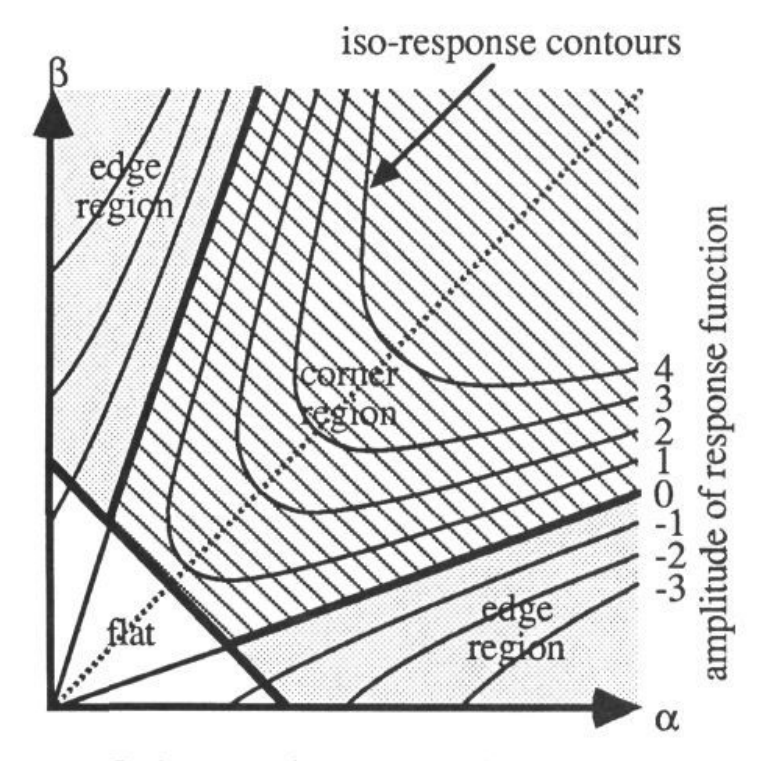
\includegraphics[height=0.25\pdfpageheight]{../Images/structure_tensor.png}
    \caption{Visualisation of distinction of image features using the eigenvalues of the structure
        tensor. $\alpha, \beta$ are equivalent to the eigenvalues $\lambda_1, \lambda_2$. Source: \cite{harris88}}\label{fig:Structure}
\end{figure}
There are several approaches to find out which case applies at the current position. The biggest
challenge here is to differentiate between edges and corners, i.e. we have to find out whether both
eigenvalues are meaningfully larger than 0 and if one is larger than the other.\\
The most intuitive approach is the one by Tomasi and Kanade, sometimes also called Shi-Tomasi
corner detector. It simply compares the smaller eigenvalue against some artificial
threshold. The set of local maxima is then the set of corners for the image\cite{shitomasi94}.
However, this approach requires to compute both eigenvalues and can thus be fairly expensive.\\
\TODO{Find sources for Rohr and Förstner}
A cheaper approach would be to either threshold the trace \[tr(\mathbf{J}_\rho) := j_{1, 1} + j_{2,
        2} = \lambda_1 + \lambda_2\] as proposed by Rohr, 1987 or the determinant \[det(\mathbf{J}_\rho) := j_{1, 1}j_{2, 2} -
    j_{1, 2}^2 = \lambda_1\lambda_2\] as proposed by Harris and F\"orstner, 1988 and 1986
respectively\cite{harris88}. Both of these approaches do not need to explicitly compute the eigenvalues of
the structure tensor and are thus not as computationally invested. Another difference between both 
approaches is that the first one requires the trace by itself to be a local maximum whereas in the
second approach, $(det(\mathbf{J}_\rho))/(tr(\mathbf{J}_\rho))$ needs to be a local maximum.\\

For the detection of relevant corners in the data selection phase, I mainly used the approach of F\"orstner/Harris as well as
the approach of Rohr even though the Tomasi-Kanade approach was an option and has also been
tested as we will see later in chapter \ref{ch:Results}. However, it has not proven as successful
as the other two methods during the initial testing phase.
%%%%%%%%%%%%%%%%%%%%%%%%%%%%%%%%%%%%%  Diffusion %%%%%%%%%%%%%%%%%%%%%%%%%%%%%%%%%%%%%%%%%%%%%%
\section{Diffusion}\label{sec:Diffusion}
Diffusion as a concept can be found basically everywhere ranging from an ink droplet in water to
distribution of heat from heating elements in a common living room but also in image processing.
The premise is fairly simple: create an equilibrium of concentration of some sorts without the violation of the principle of
mass conservation.
This equilibrium is usually achieved via the so called \textit{flux}. The flux is proportional to
the inverse direction of the highest increase in concentration, i.e. it determines the direction in
which the concentration has to ``travel'' in order equilibriate the change in
concentration\cite{weickert96}.
As a metaphor, imagine wind flowing from high to low pressure regions to balance out the difference
in air pressure. In this example, the flux describes the direction and strength of the wind flow.
\subsection{Mathematical background}
To derive the diffusion equation, we first need Fick's law \eqref{eq:Fick} that introduces the
flux
\begin{equation}
    \boldsymbol j = -\boldsymbol D\cdot\boldsymbol\nabla u\label{eq:Fick}
\end{equation}
In this equation, $\boldsymbol D$ is the \textit{Diffusion tensor}, a $2\times2$ symmetric and
positive definite matrix and $j = (j_1, j_2)$ is the aforementioned flux.\cite{dic18-02}\\
The principle of mass conservation in general is given by the equation
\begin{equation}
    \partial_t u = - \textnormal{div}(j)\label{eq:Conservation}
\end{equation}
where $u: [0, \infty) \times \Omega \rightarrow \mathbb{R}$ is a function of time and space, div
is the \textit{divergence operator}
\[\textnormal{div}(j) := \partial_x j_1 + \partial_y j_2\]
and $j$ the flux defined in~\eqref{eq:Fick}.\\
To see why this models the conservation of mass quite nicely, we have to understand what the
meaning of the divergence operator is.
In simple terms, div($u$) tells us how much the value of $u$ at a certain position changes
depending on the sign.
If we take the example from the introduction, the divergence of a region with high air pressure 
would be a positive value, since wind flows from high to low pressure regions, thus `leaving' an 
area with high pressure.
Analogously, a region with low air pressure would have a negative divergence value since it 
`takes in' wind from high pressure regions.\\
\TODO{Explain flux+divergence and conservation of mass}


\eqref{eq:Fick} and \eqref{eq:Conservation} together then form the general \textit{diffusion
    equation} or \textit{heat equation}\cite{dic18-02, weickert96}
\begin{equation}
    \partial_t u = \textnormal{div}(\boldsymbol D\cdot\boldsymbol\nabla u)\label{eq:Diffusion}
\end{equation}

Depending on the diffusion tensor we can distinguish between different types of diffusion
processes:
\subsubsection*{Linear isotropic diffusion}
In this first and simplest case, the diffusion tensor is omitted completely since it is equivalent
to the identity matrix, i.e. the diffusivity is the same across the whole image.
The consequence for the smooting process is that it is the same everywhere in the image, which
is why this type of diffusion is also often referred to as \textit{homogeneous diffusion}.
The characteristic diffusion equation in this case boils down to the 2D \textit{heat equation}
\begin{equation}
    \partial_t u = \Delta u = \textnormal{div}(\boldsymbol\nabla u)
\end{equation}
which can be solved analytically. Its solution is equivalent to a Gaussian convolution
hence explaining the homogeneous smoothing. Even though this is a nice property and this case is
completely understood in a mathematical sense, it is not very useful if one wants to e.g. enhance
edges in an image. To achieve something like this, we have to look into nonlinear methods.

\subsubsection*{Nonlinear isotropic diffusion}
The huge difference to the linear isotropic case is the diffusivity function.
Previously, we had a constant diffusivity, which resulted in the same amount of smoothing at every location.
Now we want to smooth some regions more than others, i.e. the diffusivity function depends on the
image or rather the gradient magnitude of the image. The most famous approach for this case is the
one by Perona and Malik \cite{perona-malik}.
\begin{equation}
    \partial_t u = \textnormal{div}(g(\lVert\boldsymbol\nabla u\rVert_2^2)\boldsymbol\nabla u)
\end{equation}
where
\[g(s^2) = \frac{1}{1 + s^2/\lambda^2}\]
\subsubsection{Nonlinear anisotropic diffusion}

\section{EED-based inpainting}
\TODO{Shortly explain "normal" inpainting}
\TODO{Explain basics of EED inpainting}
